\section{Измерения}

%На данный момент были проведены два текстовых измерения детектора NeuRad на территории ОИЯИ. Их целью было определение энергетического и временного разрешения детектора. В обоих экспериментах использовался прототип NeuRad. 

Первый эксперимент для определения временных характеристик детектора NeuRad был проведён в декабре 2016\,г на территории ОИЯИ. Основной  целью которого было определение временного разрешения детектора. В эксперименте использовался так называемый прототип NeuRad.

Чувствительной частью прототипа детектора служил пучок из 256 оптических волокон, сделанных из того же материала, что и в детекторе NeuRad, сечением 3$\times$3\,мм$^2$ и длиной 25\,см. и прикреплённые с одной либо двух сторон мультианодные ФЭУ (см. Рис.~\ref{ris:neuradfibers}).

\begin{figure}[!ht]
		\centering
		\begin{tabular}{cc}
			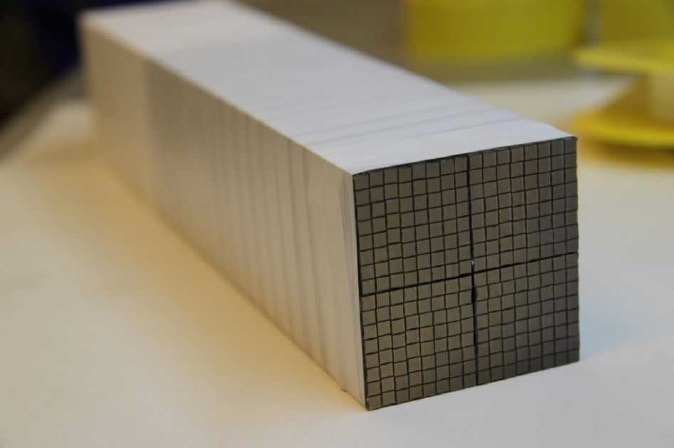
\includegraphics[width=0.52\linewidth]{neuradfibers.png} 
			&
			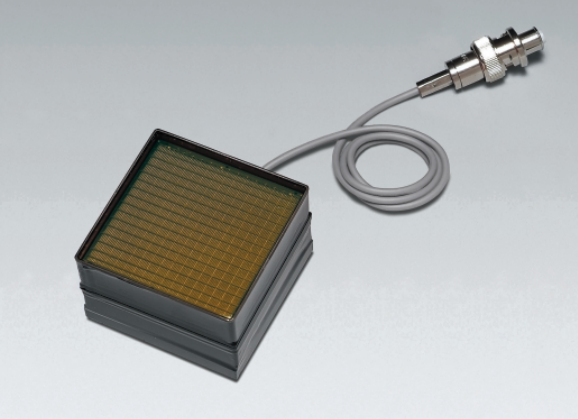
\includegraphics[width=0.48\linewidth]{H9500.png} \\
			а) & б)
		\end{tabular}
%		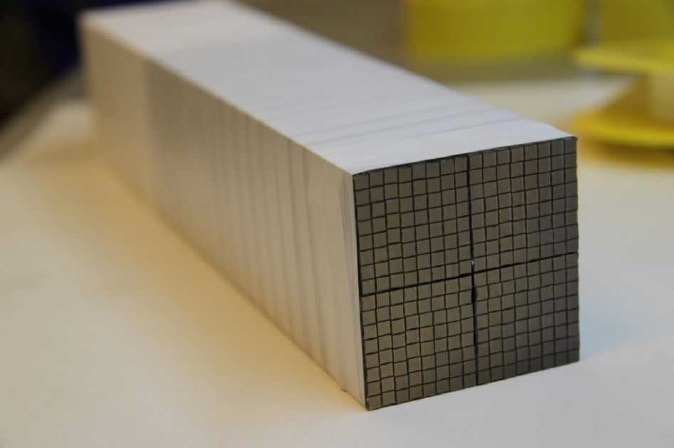
\includegraphics[width=0.5\linewidth]{neuradfibers.png}
		\caption[Short caption for list of figures]{а) Прототип NeuRad длиной 25\,см, состоящий из 256 оптических волокон. б) Мультианодный (256 анодов) фото-электронный умножитель HM9500.}
		\label{ris:neuradfibers}
\end{figure}

Для проверки качества и правдоподобности полученных результатов экспериментов в ОИЯИ, были также проведены вспомогательные измерения на территории института GSI с использованием более простого и компактного оборудования.

\subsection{Тесты временных характеристик прототипа NeuRad}
\label{sec:timeTests}
 
%\red{Временное разрешение детектора определяется как минимальное время, которое должно разделять два импульса, чтобы они были зарегистрированы как два отдельных события \cite{vratislav}. }
Изучение временных характеристик NeuRad проводилось с помощью источника гамма квантов $^{60}$Co.
Прототип, описанный выше, был помещён в чёрный ящик и облучался коллимированным пучком с энергией $E^{(1)}_{\gamma}$=1173\,кэВ и $E^{(2)}_{\gamma}$=1333\,кэВ (см. Рис.~\ref{ris:neuradexp}). Коллимитором пучок гамма гвантов был направлен на середину прототипа. Фотоны испытывали преимущественно комптоновское рассеяние на электронах материала оптических волокон. Электроны отдачи, в свою очередь, взаимодействуя с материалом волокна, возбуждали молекулы сцинтиллятора и порождали сцинтилляционные вспышки внутри оптического волокна, тем самым замедляясь. Фотоны, отражаясь от границ волокна, достигали фотоэлектронных умножителей (ФЭУ), модели HM9500, прикреплённых с торцов прототипа. 
ФЭУ были прикреплены к сборке таким образом, что площадь фотокатода соответствующая одному аноду полностью перекрывала торец одного волокна.



\begin{figure}[!ht]
	\centering
	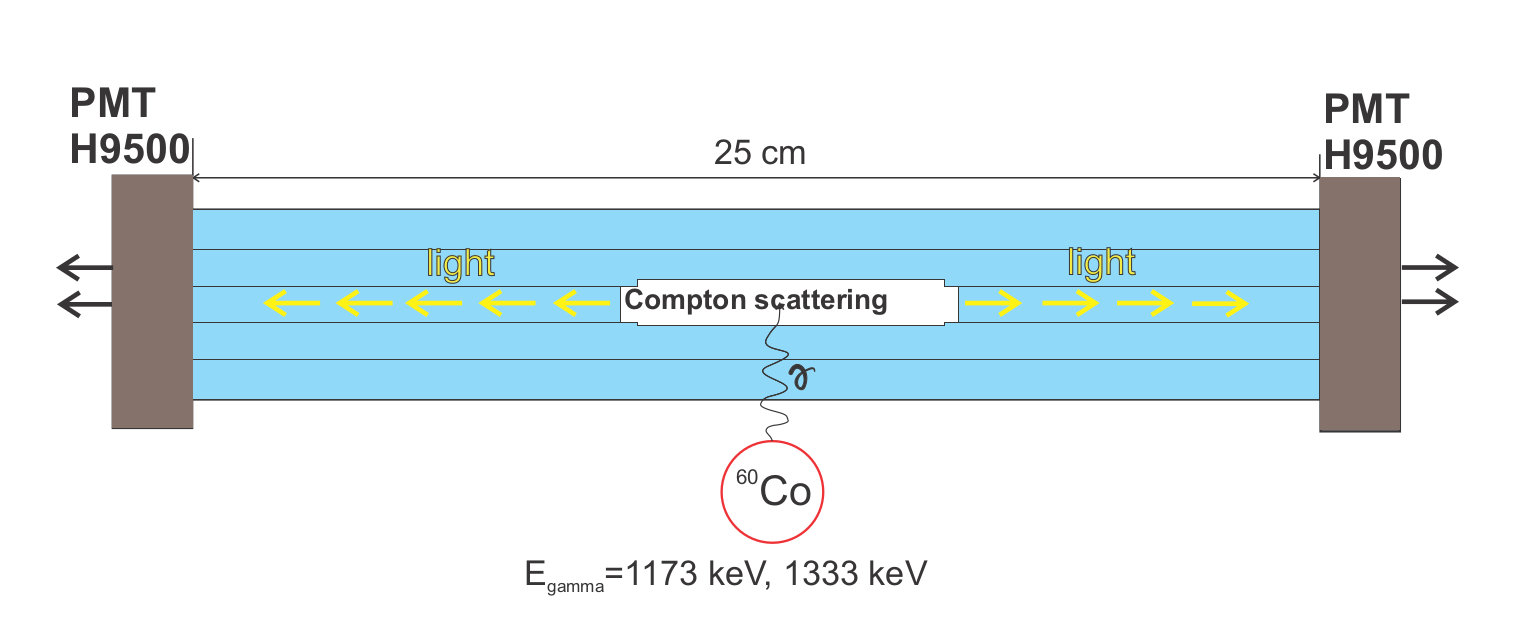
\includegraphics[width=1\linewidth]{NeuRadexperiment.png}
	\captionof{figure}{Схема эксперимента с прототипом NeuRad.}
	\label{ris:neuradexp}
\end{figure}

Для оценки временного разрешения детектора, нам было достаточно данных, взятых из одного оптического волокна. 
Полученные анодные сигналы с ФЭУ оцифровывались при помощи четырёхканального осциллографа Tektronix MSO7354 \cite{tektronix} и преобразователя DRS4 \cite{plata}.
Система работала таким образом, что данные записывались при условии, что амплитуда сигнала в выбранном канале превышала определённое значение (самотриггерование).
При выполнении этого условия, оцифровывающее устройство записывало форму сигнала в определённом временном окне, в нашем случае равном 200нс (140 нс до превышения порога и до 60 нс после), в бинарный (для DRS4) или текстовый (для осциллографа Tektronix) файла в память внешнего диска. 
Было сделано несколько сессий сбора данных, в каждом из которых были записаны 10000 сигналов с каждого ФЭУ.


Учитывая низкую интенсивность источника, можно было быть уверенным, что сигналы полученные с одного оптического волокна в рамках временного окна, данного считывающем устройством, относятся к одному событию.
Событием в данном случае будем называть однократное взаимодействие налетающей частицы с материалом детектора.

В левой части Рис.\ref{ris:signal1} показан типичный записанный сигнал. Во время измерения наблюдалось, что форма сигнала непостоянная. Можно видеть, что в данном временном окне, мы видим только один сигнал. В правой части рисунка, показана увеличенная интересующая нас часть того же сигнала.
\begin{figure}
	\centering
	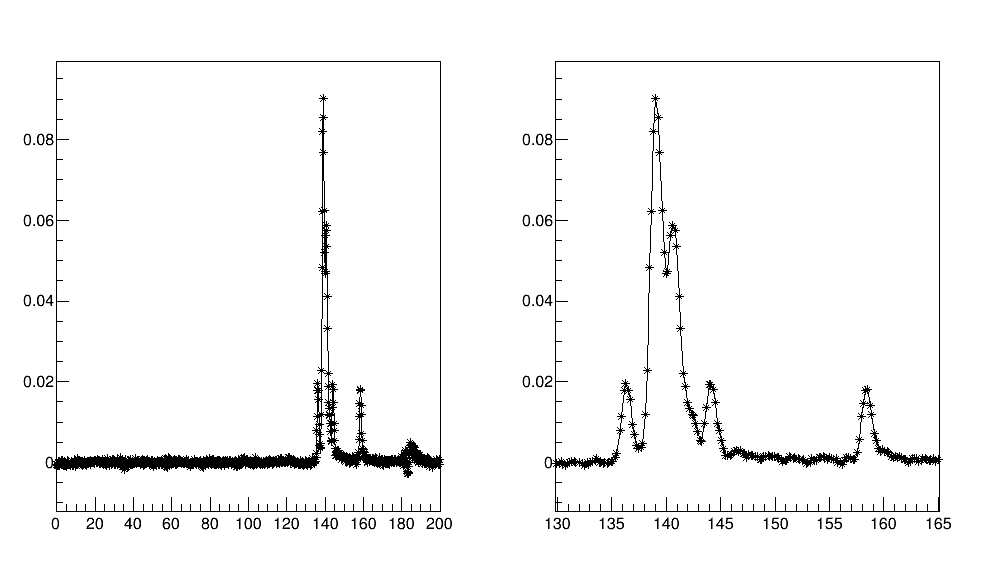
\includegraphics[width=1\linewidth]{signal1.png}
	\caption{Сигнал, полученный с одной стороны волокна.}\label{ris:signal1}
\end{figure}

С помощью алгоритмов, описание которых содержится в главе \ref{section:processing}, можно получать время прихода сигнала из его формы. 
Так, как в тестах прототипа пучок падающих частиц был коллимирован, то участок волокна, где происходило взаимодействие был заранее известен.
Ширина этого участка определяется размером отверстия коллиматора и в наших измерениях составляла 3\,мм.



\subsection{Измерения в GSI}
\label{sec:timeTestsGSI}
Для проверки качества и правдоподобности собранных данных в эксперименте с прототипом NeuRad в ОИЯИ были проведены измерения на базе лаборатории GSI в феврале 2017\,г. Схема эксперимента была похожей на ту, которая описана в главе \ref{sec:timeTests}.
Разница заключалась в том, что вместо пучка оптических волокон чувствительная часть детектора состояла из пластины сцинтиллятора (BCF12) размерами 50мм$\times$50мм$\times$4мм.С двух граней пластины, размерами 50мм$\times$50мм крепились ФЭУ. Из-за пренебрежимо маленькой толщины сцинтиллятора можно считать, что продольная координата образования световой вспышки фиксирована, и следовательно, не было необходимости коллимировать пучок. 
Также, в силу небольшой толщины чувствительной части детектора, неопределенность продольной координаты образования световой вспышки стремится к нулю, тогда и неопределённость по времени, связанное с  ней также пренебрежимо мало, см. формулу \ref{eq:distance}. Поэтому, основной вклад во временное разрешение установки вносит разрешением ФЭУ. 
%Из таблицы Таб.~\ref{tab:bolts} видим, что неопределенность по времени самого ФЭУ $\sim$0.5\,ns. 
%Мы должны достичь такого уровня неопределенности.

Детектор облучали с помощью источника $^{137}$Cs. Вспышки света в сцинтилляторе собирались ФЭУ HM9500 с двух противоположных широких граней сцинтиллятора (см. Рис.\ref{ris:gsiexp}). Сигналы с ФЭУ оцифровывались при помощи четырёхканального осциллографа Le Croy. Формы записанных сигналов качественно не отличались от сигналов, полученных в эксперименте с прототипом NeuRad, описанном в главе\,\ref{sec:timeTests}. 

%см. Рис.\ref{ris:gsiexp}. 

\begin{figure}[!ht]
	\center{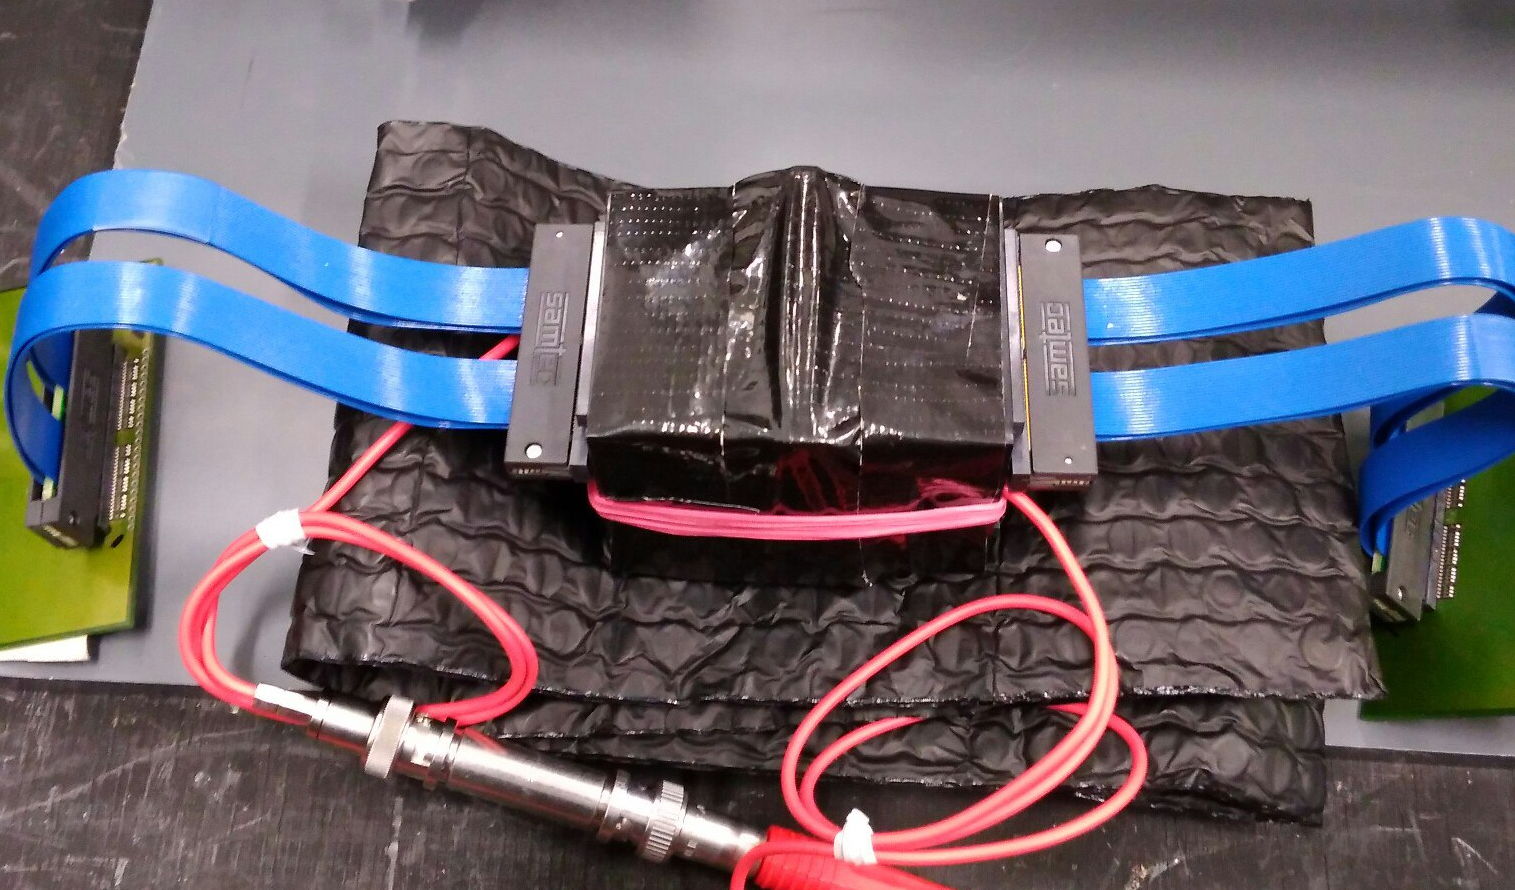
\includegraphics[width=0.5\linewidth]{gsiexp.png}}
	\caption{Экспериментальная установка измерений в GSI.}
	\label{ris:gsiexp}
\end{figure}

%В силу небольшого размера чувствительной части детектора, сигналы на выходе с осциллографа ожидались менее размытые, так как вероятность наложения сигналов порожденных сцинциляционными вспышками и их многократными переотражениями практически исключалась. 

%\subsection{Тесты энергетических характеристик прототипа NeuRad}
%
%\red{Первый временной тест прототипа NeuRad  был проведён в октябре 2016 года в Университете г. Вуперталь.
%Прототип NeuRad, описанный выше, был помещён в чёрный ящик и облучался \red{частицы} с энергиями \red{энергии} так как показано на рис.\ref{ris:neuradPrinciple}, испущенными источником $^{137}$Cs.  }